\newcommand{\checkbox}[1]{\item[$\square$]\textbf{#1}\\}

\addchap{Erstsemester-Checkliste}

Für einen erfolgreichen Start in das Studium solltest du einige organisatorische Kleinigkeiten unbedingt in den ersten Wochen erledigen.
Diese haben wir dir in folgender Checkliste mit absteigender Priorität zusammengestellt.

\begin{itemize}[leftmargin=*]

\checkbox{Wohnung}
Solltest du noch keine Bleibe gefunden haben, ist Beeilung angesagt, die schönsten Wohnungen sind schnell weg.
Wenn du in den Genuss eines superschnellen Internetzugangs kommen möchtest, seien dir die Wohnheime \link{https://www.studentenwerk-dresden.de/wohnen/wohnheimkatalog} des Studentenwerks Dresden empfohlen. Alternativ bieten sich auch Portale wie \textit{WG-Gesucht} \link{https://wg-gesucht.de/} an.

\checkbox{Erstpasswort ändern}
Jeder Student erhält vom \textit{Zentrum für Informationsdienste und Hochleistungsrechnen}, kurz ZIH, einen Uni-Account, der für alle wichtigen Funktionen rund um das Studium gebraucht wird, sei es das WLAN auf dem Campus oder die Anmeldung zu Prüfungen und Lehrveranstaltungen.
Damit du diese Services nutzen kannst, musst du dein vom ZIH vergebenes Erstpasswort im \textit{Identity Manager} \link{https://idm-service.tu-dresden.de} ändern. Das Passwort findest du in deinen Imma-Unterlagen.

\checkbox{Mail Account}
Du bekommst vom ZIH zwei E-Mail-Adressen:
\textit{s1234567@msx.tu-dresden.de} und einen Alias der Form \textit{vorname.nachname@mailbox.tu-dresden.de}.
% TODO Keep this Line?
% (ältere Jahrgänge haben E-Mail-Adressen der Form \textit{s1234567\allowbreak @mail.zih.tu-dresden.de}, wundere dich also nicht, wenn du die noch siehst).
Falls dein Name an der TU Dresden bereits existiert, lautet die Alias-Adresse für Max Mustermann dann z.B. \textit{max.mustermann1@mailbox...}.
Per Webmail oder IMAP kannst du auf dein Postfach zugreifen.
Alternativ kannst du deine Mails an eine persönliche Adresse weiterleiten, damit du nichts verpasst. \\
Vor allem wichtige E-Mails von der Uni werden an diese Adressen geschickt. Sorge deshalb dafür, dass du deine Mails regelmäßig abrufst oder an eine andere Adresse weiterleitest. Weitere Informationen unter \link{https://tu-dresden.de/zih/dienste/datennetz_dienste/e_mail}.

\checkbox{BAföG-Antrag}
Die Antragsformulare findest auf den Seiten des BMBF \link{https://www.bafög.de/de/alle-antragsformulare-432.php}. Für weitere Auskünfte steht dir das Servicebüro oder dein Sachbearbeiter im Studentenwerk zur Verfügung.
Schiebe den Antrag nicht allzu lang vor dir her, da dein Anspruch frühestens ab dem Antragsmonat gilt.
Informationen zu den Sprechzeiten beim Studentenwerk gibt es hier \link{https://www.studentenwerk-dresden.de/finanzierung/servicebuero.html}.

\newpage

\checkbox{Wohnsitz anmelden}
Offiziell musst du innerhalb von zwei Wochen beim zuständigen Ortsamt \link{https://www.dresden.de/de/rathaus/dienstleistungen/wohnsitz_meldung_d115.php} deine Wohnung anmelden.
Wer seinen Hauptwohnsitz nach Dresden verlegt, kann bei der Stadt eine \glqq Umzugsbeihilfe\grqq\ in Höhe von 150\euro\ beantragen.
Informationen dazu gibt's unter \link{https://www.dresden.de/de/rathaus/dienstleistungen/c_336.php} und \link{https://www.studentenwerk-dresden.de/wohnen/umzugsbeihilfe.html}.
Wenn du deine Wohnung als Nebenwohnsitz anmeldest, musst du Zweitwohnungssteuer zahlen. Diese beträgt 10\% der Kaltmiete pro Monat. Weitere Informationen findest du beim StuRa \link{https://www.stura.tu-dresden.de/zweitwohnungssteuer} oder der Stadt Dresden \link{https://www.dresden.de/de/rathaus/dienstleistungen/c_zweitwohnungssteuer.php}.

\checkbox{WLAN}
Sowohl auf dem Campus wie auch in den Räumlichkeiten der Fakultät kannst du mit deinen Geräten ins Internet.
Das Netzwerk heißt \textit{eduroam} und bietet dir neben einem sicheren Internetzugang an unserer Uni selbiges auch an sehr vielen anderen Universitäten weltweit.
Zugang bekommst du mit deinem Login, hier ausnahmsweise in der Form \textit{sXXXXXXX@tu-dresden.de}, und deinem Passwort. Mehr Informationen findest du unter \link{https://tu-dresden.de/zih/dienste/arbeitsumgebung/zugang_datennetz}.

\checkbox{E-Meal-Karte}
Die Mensakarte gibt es während der ESE oder in den Mensen selbst für jeweils 5\euro\ Pfand.
Zusätzlich dazu benötigst du deine E-Meal-Bescheinigung, die du auf deinem Semesterbogen findest.

\checkbox{Programmierkurse}
Besonders denjenigen ohne Programmiererfahrung werden die im Wintersemester angebotenen Programmierkurse ans Herz gelegt. Insbesondere der C- und der Java-Kurs sind sehr hilfreich, um durch die ersten Semester zu kommen. 
Diese finden in der Regel unter der Woche statt, manche auch am Wochenende.
Für Details wende dich an \link{programmierung@ifsr.de} oder behalte die News auf der Seite des FSR \link{https://www.ifsr.de} im Auge.

\checkbox{(optional) Sprachkurse}
Die TU Dresden bietet Sprachkurse für Englisch und viele weitere Sprachen an. Um dein Diplom abzuschließen oder dich nach dem Bachelor in den Informatik-Master einzuschreiben, musst du Englischkenntnisse nachweisen. Die Einschreibung für die Sprachkurse wird je nach Kurs im Laufe der ersten beiden Wochen deines Studiums freigeschaltet.
Erkundige dich auf den Seiten des LSK \link{https://lskonline.tu-dresden.de} frühzeitig, wann dies ist. Die meisten Kurse sind sehr schnell voll.

\checkbox{(optional) Sportkurse}
Wie für die Sprachkurse gilt auch hier, wer zuerst da ist\ldots{} Das Angebot kannst du beim Universitätssportzentrum (USZ) einsehen \link{https://tu-dresden.de/usz}.
Hast du dich für einen Kurs entschieden und bei freigeschalteter Einschreibung für diesen angemeldet, musst du nur noch die Anmeldebescheinigung drucken und den Kostenbeitrag innerhalb von drei Tagen auf das Konto des USZ überweisen.

\newpage

% TODO Continue here

\checkbox{Studienrelevante Dokumente}
Das Vorlesungsverzeichnis und die Prüfungs- und Studienordnung erhältst du auf den Seiten des Prüfungsamtes \link{https://tu-dresden.de/inf/pra}.
Gedruckte Ordnungen gibt's beim FSR und in deiner ESE-Tüte.
Alle wichtigen Informationen zu den einzelnen Vorlesungen findest du auf den jeweiligen Seiten der Institute im Netz.
Die Professoren werden dir dazu jedoch auch noch alles in den ersten Vorlesungen mitteilen. Sonst hilft natürlich schon einmal ein Blick auf die Seite des FSR \link{https://www.ifsr.de}.

\checkbox{Bibliotheksausweis}
Bekommt man nach vorheriger Online-Anmeldung und nach Vorlegen eines Wohnsitznachweises (Personalausweis) direkt am Schalter in der SLUB (Zellescher Weg 18) \link{https://www.slub-dresden.de/service/anmelden}.

\checkbox{Fachschaftsratwahlen}
Wähle deine studentischen Vertreter im FSR Informatik.
Die Wahlen finden jedes Jahr im November statt.
Geh wählen!
Und noch besser: Lass dich wählen!

\vfill

\begin{figure}[h!]
\centering
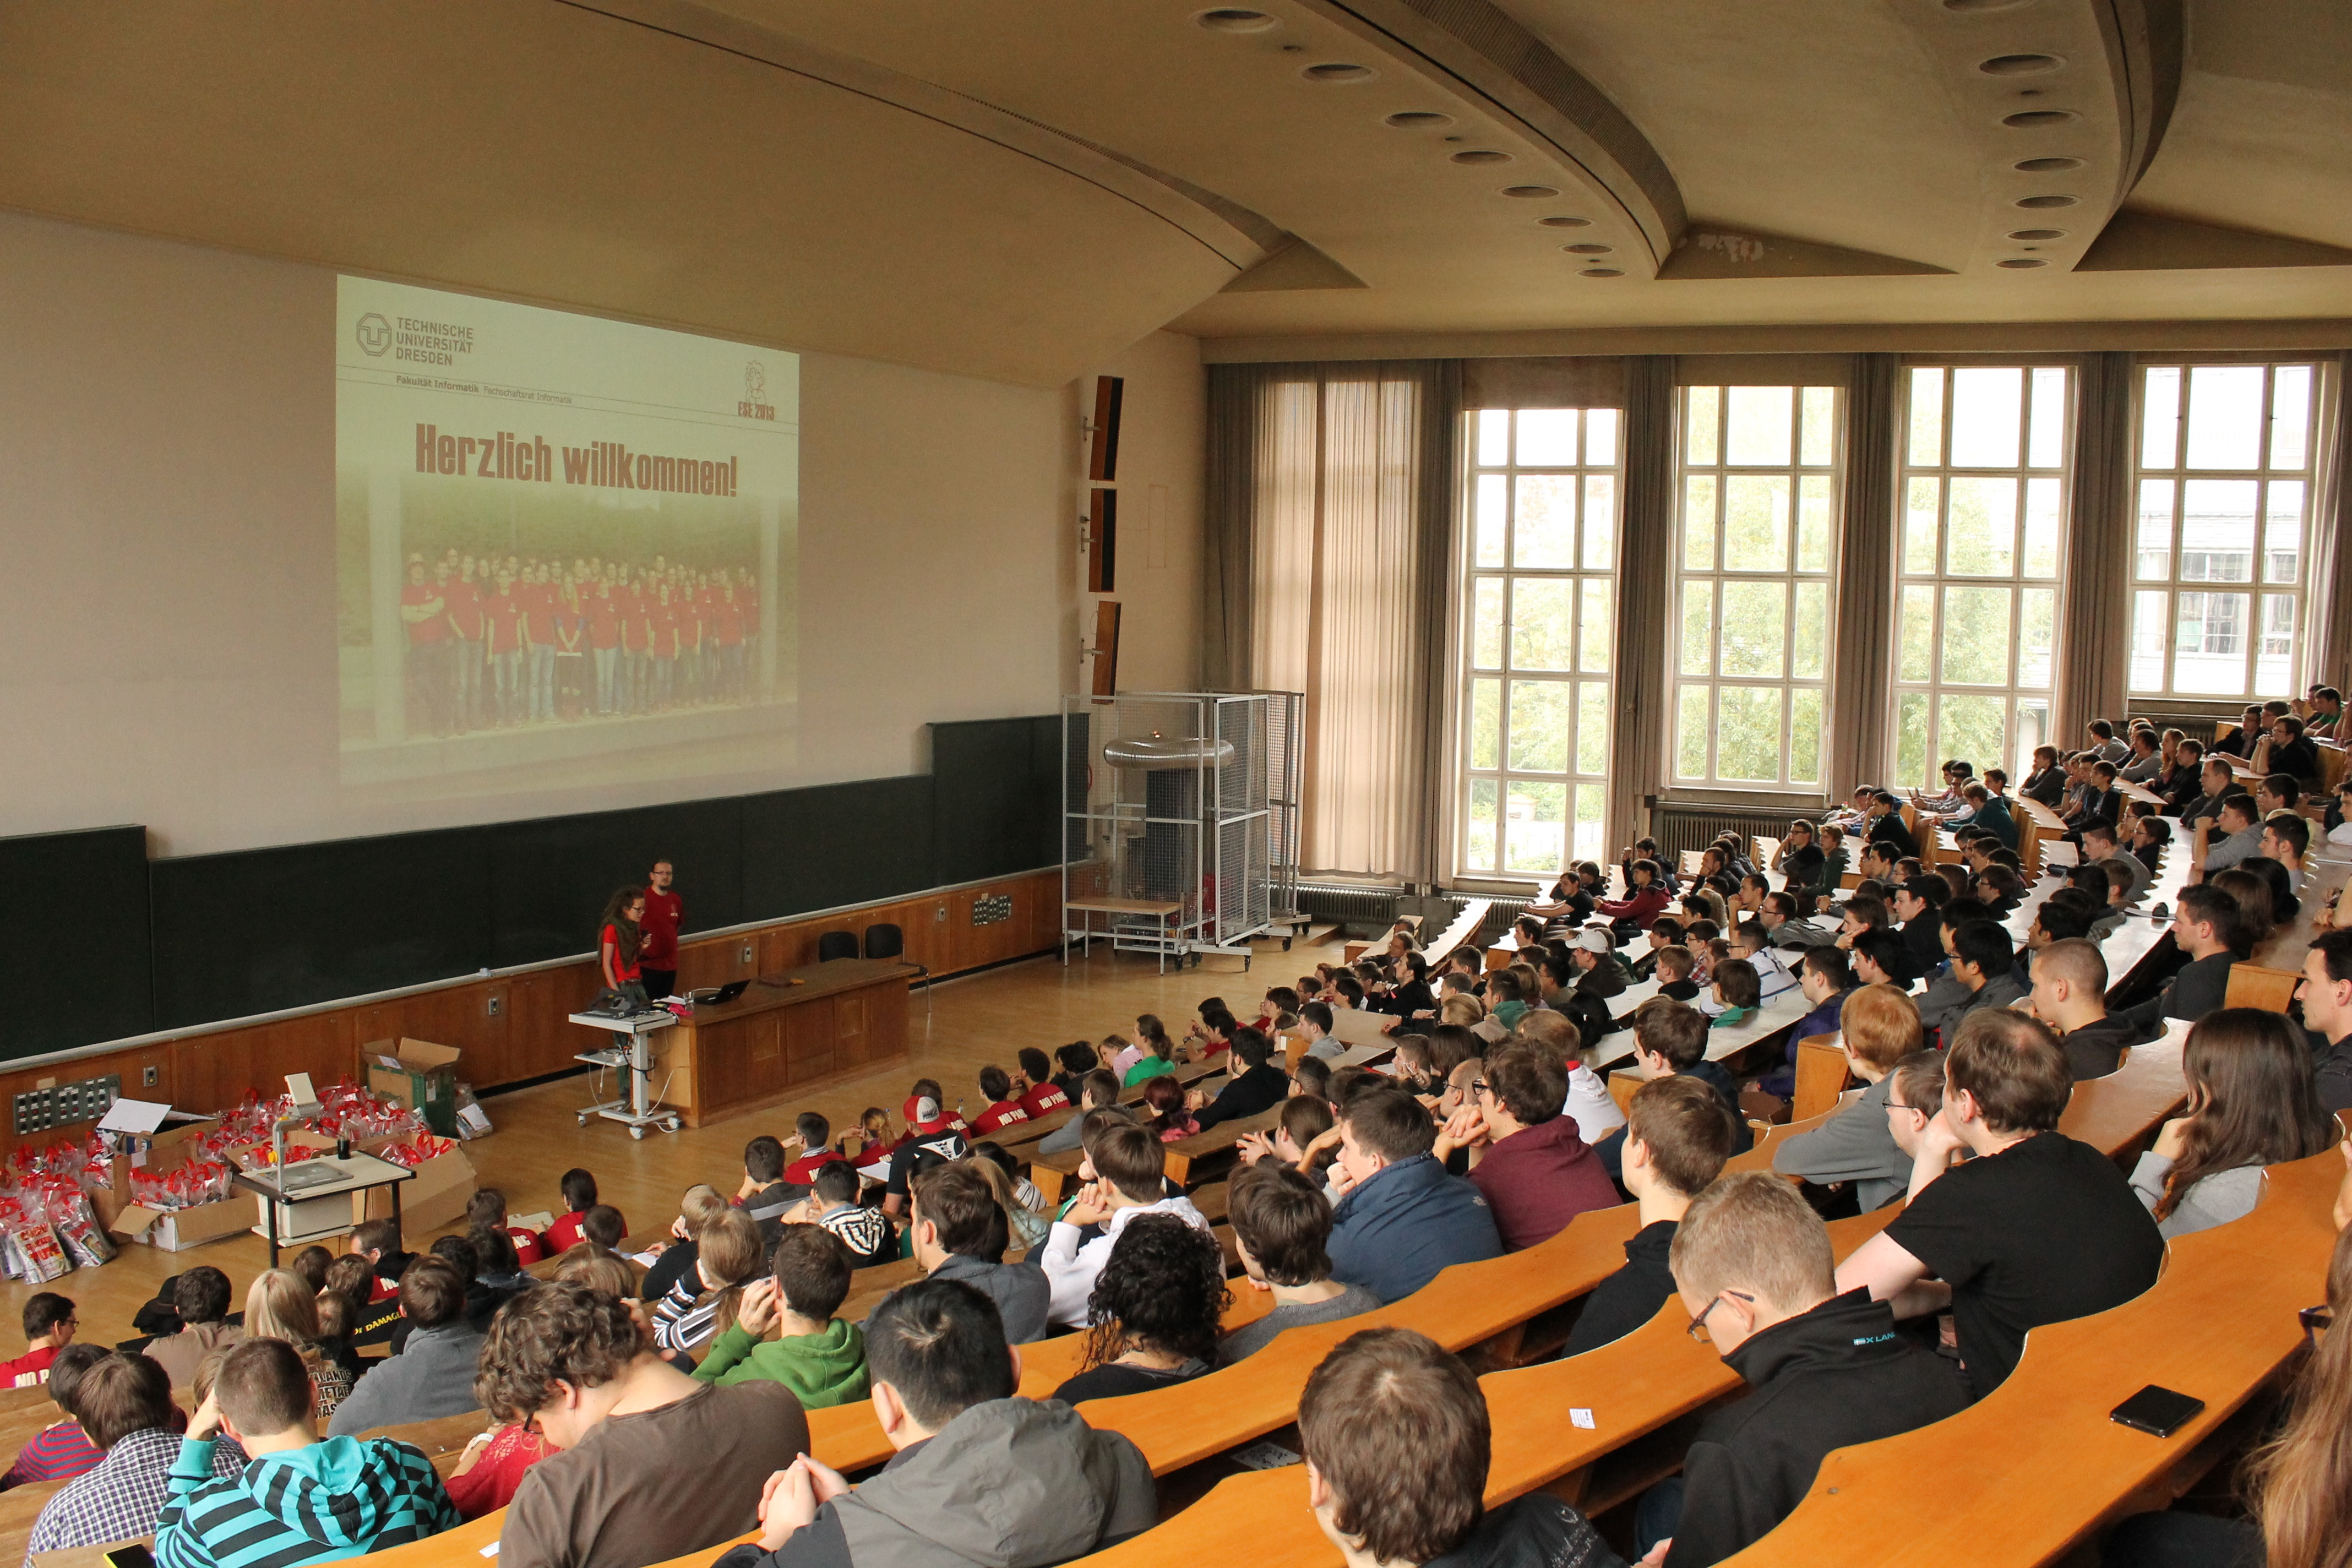
\includegraphics[width=0.9\linewidth]{img/ese2013/barschoe.jpg}
\end{figure}

\newpage


\checkbox{Prüfungseinschreibung}
% TODO: Bleibt es bei jExam oder wird das da schon Selma?
Ab Anfang nächsten Jahres kann man sich in jExam für die Prüfungen anmelden. Der Termin wird auf der Seite des Prüfungsamtes bekannt gegeben. Melde dich rechtzeitig an, denn sonst kannst du nicht an der Prüfung teilnehmen.
Schreib dich in die Prüfungen der Fächer ein, die du besucht hast.
Beachte, dass die erste Prüfung in Mathe bereits Anfang Dezember statt findet.
Viel Erfolg!

\checkbox{Rückmeldung zum Sommersemester}
Ab Mitte Januar 2016 kannst du den Semesterbeitrag für das nächste Semester überweisen.
Den genauen Betrag und Termine findest du online \link{https://tu-dresden.de/imma/rueckmeldung}.
Kümmere dich rechtzeitig darum, sonst wirst du automatisch exmatrikuliert!

\end{itemize}

\vfill

\begin{figure}[h!]
\centering
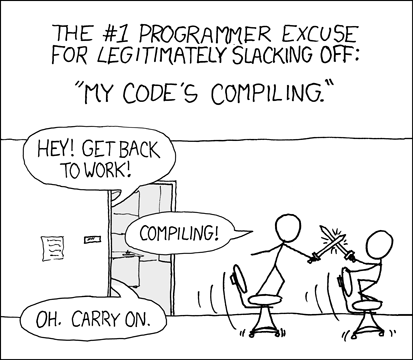
\includegraphics[scale=.4]{img/xkcd/compiling.png}
\caption*{{\small \textit{'Are you stealing those LCDs?' 'Yeah, but I'm doing it while my code compiles.'\\\hspace*{1mm}\hfill(https://xkcd.com/303)}}}
\end{figure}
